% Migrated from proposal/proposal.tex (5 October 2026) on 14 October 2026.
\chapter{Worked Example: From a Pathway to Text Codes}
\label{app:example}

This example applies the method to a constructed privacy notice of a
fictional period tracker, \emph{App~F}; it describes no real app.

\textbf{Step 1: Model the tree.} Figure~\ref{fig:example-path} adapts
Knabenhans et al.'s targeted-advertising tree (their Fig.~6c, with the
tracking sub-tree of Fig.~5b) to App~F~\parencite[\S4.2]{knabenhans2026harms}.
The components keep the paper's roles: C1 is their \emph{reveal other
attributes}, C2 a \emph{persistent identifier}, C3 \emph{online metadata},
which the paper says includes advertising IDs, C4 \emph{repeated
observations}, and C5 the \emph{digitization of data records} that enables
data brokerage. OR means one branch suffices; OR+ means several components
combine. App~F's core function, predicting the cycle, can run on the phone and
reveals nothing to an ad partner, so both branches need implementation
choices that the provider controls and can describe. Dropping the ad SDK
blocks tracking, and not keeping or not selling server records blocks
brokerage; sending interest categories instead of entries does not, because a
category such as \enquote{family planning} still carries the
pregnancy~\parencite{martin2025cookies}.

\begin{figure}[h]
\centering
\resizebox{\textwidth}{!}{%
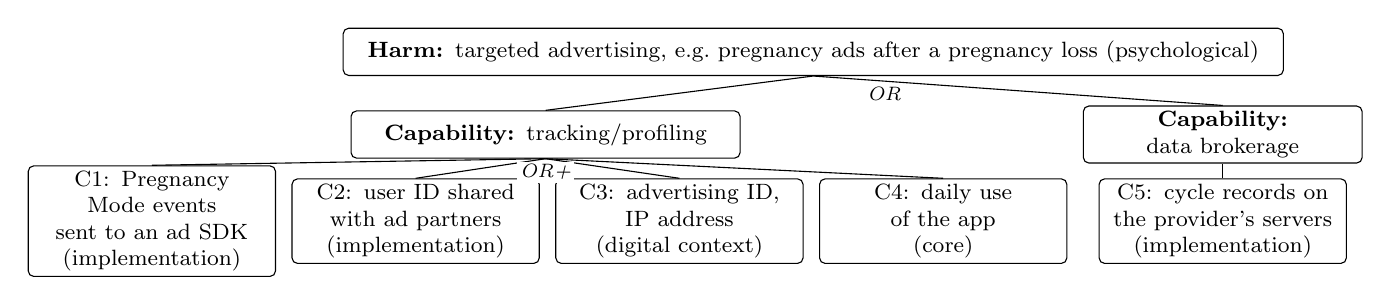
\begin{tikzpicture}[
  font=\footnotesize,
  bx/.style={draw,rounded corners=2pt,align=center,text width=30mm,
             minimum height=10mm,inner sep=2pt},
  lb/.style={font=\scriptsize\itshape,fill=white,inner sep=1pt}]
  \node[bx,text width=118mm,minimum height=6mm] (h) at (8.4,2.15)
    {\textbf{Harm:} targeted advertising, e.g.\ pregnancy ads after a
     pregnancy loss (psychological)};
  \node[bx,text width=48mm,minimum height=6mm] (t) at (5.0,1.1) {\textbf{Capability:} tracking/profiling};
  \node[bx,text width=34mm,minimum height=6mm] (d) at (13.6,1.1) {\textbf{Capability:} data brokerage};
  \node[bx] (c1) at (0.0,0) {C1: Pregnancy Mode events\\sent to an ad SDK\\(implementation)};
  \node[bx] (c2) at (3.35,0) {C2: user ID shared\\with ad partners\\(implementation)};
  \node[bx] (c3) at (6.7,0) {C3: advertising ID,\\IP address\\(digital context)};
  \node[bx] (c4) at (10.05,0) {C4: daily use\\of the app\\(core)};
  \node[bx] (c5) at (13.6,0) {C5: cycle records on\\the provider's servers\\(implementation)};
  \foreach \c in {c1,c2,c3,c4} \draw (\c.north) -- (t.south);
  \draw (c5.north) -- (d.south);
  \draw (t.north) -- (h.south);
  \draw (d.north) -- (h.south);
  \node[lb] at (5.0,0.62) {OR+};
  \node[lb] at (9.3,1.62) {OR};
\end{tikzpicture}}
\caption{App~F's version of Knabenhans et al.'s targeted-advertising tree,
read from the bottom up.}
\Description{A three-level tree. Four components, Pregnancy Mode events sent
to an ad SDK, a user ID shared with ad partners, the advertising ID and IP
address, and daily use of the app, combine (OR+) into tracking and profiling.
Cycle records on the provider's servers enable data brokerage. Either
capability (OR) can lead to targeted advertising, such as pregnancy ads after
a pregnancy loss, a psychological harm.}
\label{fig:example-path}
\end{figure}

\textbf{Step 2: Decide whether the tree applies.} The applicability record
notes the required features (C1 and C3 reach ad partners; C5 exists), the
evidence (S2, S3 below), the assumption (the shared events include Pregnancy
Mode, which the text does not state) and the decision: \emph{applicable}, so
psychological harm applies to App~F. Mentions are coded regardless;
applicability only decides which \emph{missing} harms count as gaps (RQ1).

\textbf{Step 3: Code the statements.} Each statement in Table~\ref{tab:worked}
is one unit. A: every mentioned element with its status (asserted, possible,
denied); B: a stance, only for a named harm; C: the measure's framing,
strength and scope. A dash: not applicable.

\begin{table}[h]
\centering
\begin{singlespace}
\caption{Constructed statements and their codes.}
\label{tab:worked}
\small
\begin{tabularx}{\textwidth}{@{}L{0.5cm}>{\raggedright\arraybackslash}X>{\raggedright\arraybackslash}X L{2.0cm}>{\raggedright\arraybackslash}X@{}}
\toprule
 & \textbf{Statement} & \textbf{A: What is mentioned} & \textbf{B: Stance}
 & \textbf{C: Protection} \\
\midrule
S1 & \enquote{We use your cycle entries to predict your fertile window.}
   & Entries: component, asserted. Prediction: inference, asserted (a
     feature) & -- & -- \\
\addlinespace
S2 & \enquote{Our advertising partners receive app usage events and your
     advertising ID.}
   & C1 and C3 to partners: components, asserted & -- & -- \\
\addlinespace
S3 & \enquote{We store your entries on our servers and never sell them.
     Partners only receive interest categories, not your entries.}
   & C5: component, asserted. Sale: denied. Entries to partners: denied.
     Categories to partners: asserted
   & -- & No-sale pledge (practice commitment); inferences instead of raw
     data; data-flow framing; absolute \\
\addlinespace
S4 & \enquote{Partners never see your entries, so you will never get
     pregnancy-based ads.}
   & Entries to partners: denied. Pregnancy-based ads (profiling):
     denied & -- (no harm named)
   & Inferences instead of raw data; harm framing; absolute; scope:
     pregnancy-based ads \\
\addlinespace
S5 & \enquote{Pregnancy ads can upset users, e.g.\ after a loss, but this
     rarely happens.}
   & Distress from such ads: psychological harm, possible
   & Acknowledged and qualified (how often) & -- \\
\bottomrule
\end{tabularx}
\end{singlespace}
\end{table}

\noindent\textbf{Why these codes.} S1: a prediction made for the user gives
no one else access; no harm is named, so no stance. S2: the data flow is named
but not what partners can do with it, so tracking is not coded. S4: a
capability is denied, not a harm, so no stance. S5: \enquote{rarely}
qualifies how often the harm occurs, so it carries two stances. Dismissing a
capability without naming a harm would be reassurance, not minimisation.

\textbf{Step 4: Review the protection claims.} S3's no-sale pledge covers the
brokerage branch and, taken at its word, closes it: no mismatch. Tracking lies
outside its scope, since C1 and C3 still flow (S2); S3 leaves it open without
contradicting it, which RQ3 records as data-flow framing. S4 promises no
pregnancy-based ads, placing tracking inside its scope; withholding entries
removes neither C1 nor C3, and categories still carry the pregnancy: the
author records a \emph{potential mismatch} with this reasoning. A mismatch
concerns what the text promises, not whether App~F is safe.

\textbf{Step 5: Summarise.} Psychological harm applies and is mentioned once
(S5); tracking is never named, although S2 describes its components. RQ3: one
scoped data-flow claim without mismatch (S3), one absolute harm-framed claim
with a potential mismatch (S4).
